\section{Design}\label{sec:design}

DataSeries is intended to provide streaming access to structured serial
data. Corresponding
to the first four properties\footnote{The fifth property, an expressive
programming interface, is described in Section~\ref{sec:programming}.}
described in the introduction, DataSeries was designed with the
following goals in mind. First, it should be very storage
efficient. Second, it must be efficient to encode, decode and
interpret the data.  Third, the format should not constrain the
types of information to be stored. Fourth, the internal data must be
self-describing, i.e., the names and types of the data stored have to
be determined by the contents of the file itself, rather than 
externally.

\subsection{File structure}\label{sec:structure}

\begin{figure*}
% \vspace{-0.6cm}
\hfil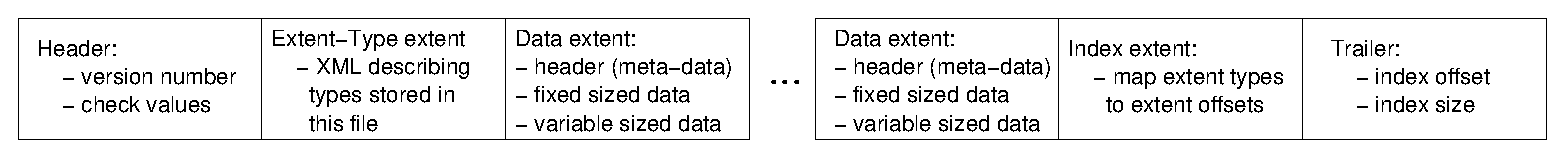
\includegraphics[width=6.5in]{fig/ds-format2.eps}\hfil
\caption{Internal structure of a DataSeries file.}
\label{fig:dsorg}
% \vspace{-2mm}
\end{figure*}

DataSeries' data model is conceptually very similar to that used
by relational databases. 
Logically, a DataSeries file is composed of an ordered sequence of
{\it records}, where each record is composed from a set of {\it
fields}. Each field has a {\it field-type} (e.g., integer, string, double,
boolean) and a name. A DataSeries record is analogous to a row in a
conventional relational database. We call the type of a row 
the {\it extent-type} because 
an {\it extent} contains a collection of rows with the same fields and 
field-types.

A single DataSeries file comprises a
collection of extents (potentially with different extent-types), plus a
header and extent-type extent at the beginning of the file, and an index extent and
trailer at the end of the file. Figure~\ref{fig:dsorg} shows
this organization.  The extent-type and index extents are the same as the
other extents in the file except that their names and extent-types are 
hard-coded in the library.

The header on a DataSeries file contains the DataSeries file version,
and five check values 
to determine the encoding format for integers and doubles.
DataSeries files
are always written out using the native formats of the system doing
the writing. We did this to minimize byte-swapping overheads,
as usually the architecture reading the files is the same 
as the architecture writing the files.
The library transparently does endianness conversions in the 
rare circumstances that this is not true, and also provides a ``repack''
utility for explicit conversion.

Immediately following the header is the extent-type extent. Records in
this extent have a single string-valued field, each of which 
contains an XML specification that defines the extent-types of all the 
other extents in the file.  

% TODO: get the xml figure example working again.

% Figure~\ref{fig:xml} shows an example of the XML used to describe an extent-type.
% \begin{figure}
%  \vspace{-0.6cm}
% \hfil
% \includegraphics[width=2.8in]{fig/xml.eps}
% \hfil
% \caption{Example XML used to describe extent types, as described in
% Section~\ref{sec:structure}. Section~\ref{sec:extenttype} discusses
% extent typing while Section~\ref{sec:options} describes the opt\_* and
% pack\_* options. }
% \label{fig:xml}
% % \vspace{-2mm}
% \end{figure}

When reading a DataSeries file, the trailer is read next.  It consists
of the offset and size (after compression) of the index extent.  The
offset is used to read the index extent, which has two fields, an
extent-type and an offset, to allow direct access to extents of a single type.
The index and trailer are
stored in this order, at the end of the file, to enable efficient
writing. The writer will often not know, a priori, what the final
extent sizes will be, so space for the index cannot be allocated until
after the extents have been written.

The data extents themselves consist of a header, followed by the 
fixed size data
and the variable sized data.  Both fixed and variable sized data may be
compressed, using any one of a number of standard compression
algorithms~\cite{GZIP,BZIP,LZF,LZO}.  The header contains metadata
about the data in the extent, such as the compressed sizes of the
fixed and variable data, the number of records in the extent, the
uncompressed size of the variable length data, the compression mode,
the extent-type of the extent, and checksums of the extent before and
after compression to guard against hardware and software errors.
Checksum validation can be disabled during extent reading to improve
performance at the cost of reduced reliability.

Each row in the fixed size data is stored as a structure, with the fields sorted by size and with 
padding between sizes.
In particular, in each row, all of the boolean fields are packed, then all
the byte fields, padding is added to align to a 4 byte boundary, and
then the 4 byte integer and variable offset pointers are packed.
Lastly, the structure is padded to an 8 byte boundary and the 8 byte
integer and double fields are packed. When uncompressed, this layout
allows for very efficient access to data: every field can be accessed
through a pointer to the row, using a single addition and deference. 
This access method achieves goal two -- efficient decoding and
interpretation of the data.

\subsection{Extent types and options}\label{sec:extenttype}

An extent-type in DataSeries defines the field-type of all the fields in a
related group of records.  Every extent-type has a name; this is
intended to be a general description of the record.  We have found that
using a naming convention that encodes type and hierarchical information,
such as 
Trace::BlockIO::HPUX, 
Trace::NFS::common or
Trace::NFS::read-write
%, or 
%\linebreak[4] Summary::Network::IP::bandwidth-rolling
works well, providing information to the user on what is contained, and 
about extents that may be related (e.g., the Trace::NFS::* names above). 
% NFS::common and
% \linebreak[4] NFS::read-write). 
The extent-type also has a namespace to avoid naming conflicts between
organizations and a version number to make it easy to test whether
a program is compatible with a particular extent-type.
% We previously used a format with spaces in it, but
% found this was inconvenient to use with command line tools.  
% INCLUDE IN EXTENDED VERSION
%% To handle
%% the case where different organizations happen to use the same
%% name, each extent type also has a namespace which is intended to be a
%% domain or host name and has the semantics that two people who
%% independently choose names will choose different namespaces.  
%% Finally,

% Update ExtentType.hpp if you change this.

The extent type also has a version number of the form major.minor with the
semantics that minor versions are only allowed to add new fields,
whereas major versions can remove fields, rename fields or change
field semantics.  This means that analysis code that can process
version 1.x will work on any version 1.y for y $\geq$ x, but may or may not
work on version 2.0.

\subsection{Data types}

DataSeries currently supports six data types:
\textbf{bool} (0 or 1),
\textbf{byte} (0-255),
\textbf{int32} (signed 32bit integer),
\textbf{int64} (signed 64bit integer),
\textbf{ double} (IEEE 64 bit floating point), and
\textbf{variable32} (up to $2^{31}$ bytes\footnote{This could be changed to $2^{32}$ bytes by use of unsigned instead of signed.} of variable length data, such as strings).
% This is typically used for recording string values.

Supporting additional data types is a straightforward extension that
does not require changing the version of DataSeries.  In practice we
have found these data types to be sufficient.
% for the many types of data we have stored.  
%Section~\ref{sec:lessons} discusses some possible extensions.

\subsection{Options}\label{sec:options}

In addition to the types that are supported, there are a number of
options that can be applied to the data types.  Options are either of
the form opt\_*, or pack\_*; the former extend or change the values
available to applications, and require applications to understand the
option, whereas the latter form are transparent to applications, but
enable higher compression than would otherwise be available. Options
are applied to either an entire extent or to individual fields.  One
possible direction for future work would be automatically inferring
the ``best'' packing options.

\subsubsection{Extent-level options}
\label{sec:design:extent-options}

Extent level options control the way the entire extent is stored.
Currently there are three options here:

\begin{enumerate}

\item pack\_null\_compact: Should we remove all of the nullable fields
before running the results through compression.  For records with many
nullable values this can greatly increase the compression ratio at a
cost of additional computation time.  See section~\ref{sec:ellard} for
an evaluation of this option.

\item pack\_pad\_record: This option controls how the record is
padded.  Originally all records were padded to 8 bytes.  For records
with only 4 byte or smaller fields, this wastes some amount of space,
and hence the option to pad to the maximum column size was added.  See
section~\ref{sec:world-cup-1998} for an evaluation of this option.

\item pack\_field\_ordering: This option controls how the fields are
ordered within a record.  It turns out some files compress better with
different field orderings.  See section~\ref{sec:world-cup-1998} for
an evaluation of this option.

\end{enumerate}

\subsection{Field-level Options}
\label{sec:design:field-options}

Field-level options control the meaning of individual fields (for
opt\_* options), or how that field is represented before compression
(for pack\_* options).  Options include:

\begin{enumerate}

\item opt\_nullable: Indicates values in this column can be null.
This option is
implemented by generating a hidden boolean column that determines if
the value is null.

\item opt\_doublebase={\it base-value}: Specifies a relative base for
doubles.  This is used to gain additional precision in the double
without losing the absolute value.  
This is particularly useful for storing Unix time stamps with nanosecond
precision. In particular, we have found this
useful for storing time in seconds in Unix time\footnote{Unix time has an epoch
start of 12AM, 1 January 1970.}, but with a precision in nanoseconds, which
would otherwise be impossible as an IEEE double has insufficient
precision.

\item pack\_scale={\it scale-value}: This specifies the precision to use for
double values; in particular it means that the double will be
multiplied by 1/{\it scale-value}, and rounded to an integer before
being compressed, with the reverse transform applied after the data is
uncompressed.  This option is useful because values that are stored as
doubles sometimes accumulate pseudo-random bits in the low
digits.  These pseudo-random bits contain no useful information and
reduce the achievable compression.
This option improves compression by removing the pseudo-random bits in the low 
bits of doubles by scaling and rounding the double.  

\item pack\_relative={\it field-name}: Specifies that this field
should be packed relative to another field.  This delta encoding
option is useful for compressing time stamps and other values which
may be large but are usually close to the previous value in the same
field or the value of a different field in the same row.  In
particular it means that if {\it field-name} is the same as the
current field's name, the previous row's value will be subtracted from
the current row's value before the data is compressed, and otherwise
from the value of the other field in the same row.  This feature is
only supported for int32, int64, and double fields.  For double fields
it is required that the fields be packed with pack\_scale as well to
eliminate precision issues.

\item pack\_unique: Specifies that each unique variable32 value
should only be packed once within that extent.  This option applies across all variable32
fields with pack\_unique enabled.  For fields with many repeated
values this option can significantly increase the effective
compression ratio because it entirely removes duplicate data within that extent
(compression algorithms only remove it partially).

\end{enumerate}

\subsection{Design summary}

The DataSeries file format was designed to allow for flexibility
(through the use of a self-contained and extensible type description
for extents) and performance (through extensive use of compression and
a data layout that allows for direct access to data values). 
Section~\ref{sec:results} describes experiments using
DataSeries that quantitatively validate these claims.


% TODO: add something about time formats in here; include http://cr.yp.to/libtai/tai64.html

